\documentclass[12pt]{article}
\usepackage[margin=1in]{geometry}
\usepackage{hyperref}
\usepackage{enumitem}
\usepackage{titlesec}
\usepackage{parskip}
\usepackage{graphicx}
\titleformat{\section}{\large\bfseries}{\thesection.}{1em}{}
\titleformat{\subsection}[runin]{\bfseries}{\thesubsection.}{1em}{}[.]

\title{WeRideTransit Fare System Development Proposal}
\author{Submitted by: Harley Glayzer\\
Independent Developer, Rapid City, SD}
\date{\today}

\begin{document}

\begin{minipage}{0.3\textwidth}
    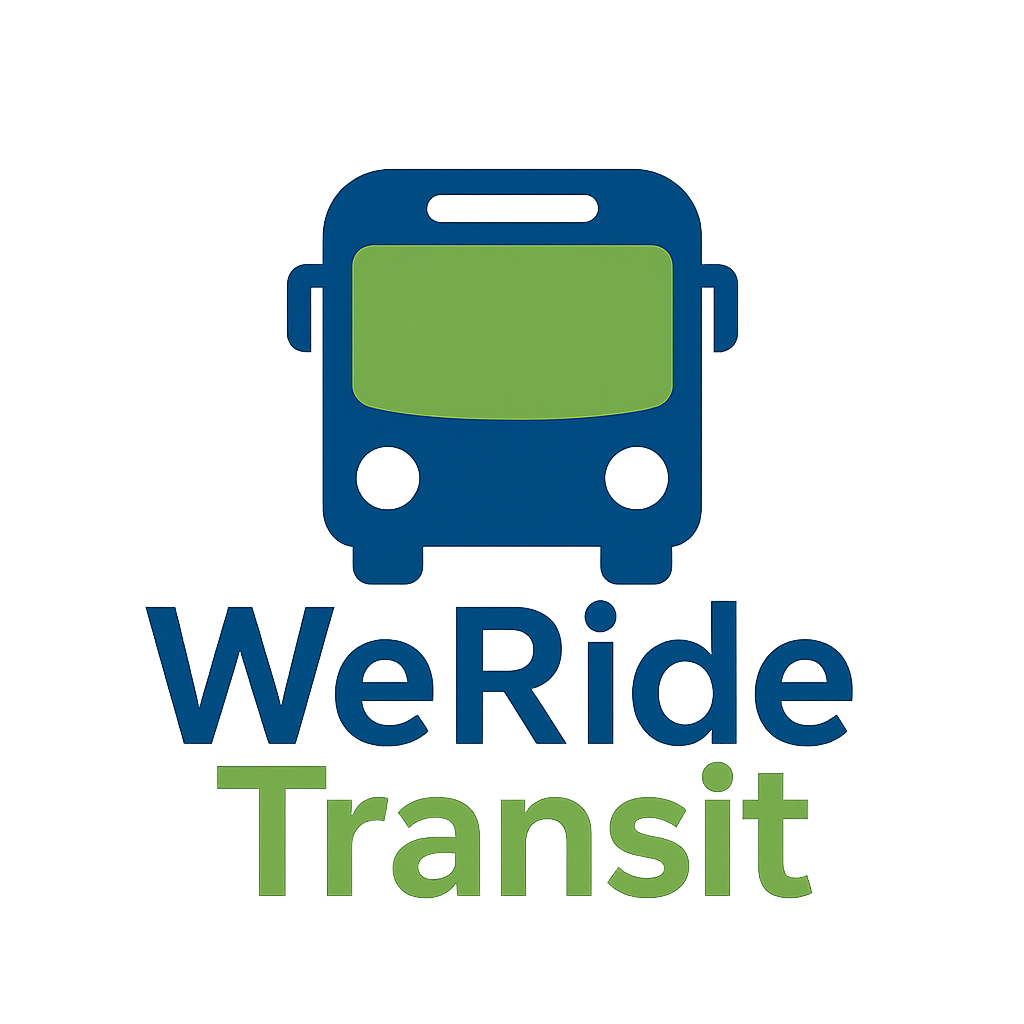
\includegraphics[width=\textwidth]{WeRideTransit_vertical.png}
\end{minipage}
\hfill
\begin{minipage}{0.65\textwidth}
    \centering
    {\Huge\bfseries RapidRide Proposal}\\[0.5em]
    {\large July 2025}
\end{minipage}
%\maketitle

\section{Project Summary}
WeRideTransit is a modular, secure, and open-source digital fare system designed to meet the needs of small- to mid-size transit agencies. It enables passengers to purchase fare tickets via Stripe, store them on mobile devices, and validate them using cryptographically signed QR codes. This proposal outlines the scope, completed milestones, pricing model, licensing terms, and future expansion potential.

\section{Project Scope}
This project includes the development, deployment, and maintenance of:

\begin{itemize}[itemsep=0.5em]
    \item A secure FastAPI-based backend server for user authentication, ticket generation, and validation
    \item A PySide6/QML-based frontend application with QR scanning and digital wallet functionality
    \item Stripe payment integration with webhook fulfillment
    \item Cryptographically signed tickets using Ed25519
    \item Ticket validation and single-use logic on the server
\end{itemize}

\section{Technology Overview}
\begin{itemize}[itemsep=0.5em]
    \item \textbf{Backend:} Python 3.11, FastAPI, SQLAlchemy (async), PostgreSQL/SQLite
    \item \textbf{Frontend:} PySide6, QML, OpenCV (QR scanner), QtMultimedia
    \item \textbf{Security:} Ed25519 digital signatures, OAuth2/JWT tokens
    \item \textbf{Payments:} Stripe Checkout Sessions and Webhooks
\end{itemize}

\section{Completed Milestones}
\begin{itemize}[itemsep=0.5em]
    \item Secure API for ticket generation and validation
    \item QR code payload generation and scanner integration
    \item Wallet UI and ticket list formatting
    \item Stripe payment integration and ticket issuance webhook
    \item Page-based frontend navigation with dynamic validation results
\end{itemize}

\section{Cost Estimate}
The following estimate is based on an hourly rate of \$40/hour.

\begin{itemize}[itemsep=0.5em]
    \item Initial Backend Development: \$2,500–\$3,000
    \item Frontend Application: \$1,800–\$2,200
    \item Stripe Integration and Fulfillment: \$800–\$1,000
    \item Deployment and Configuration: \$500–\$800
\end{itemize}

\textbf{Total Initial Deployment Estimate: \$5,600–\$7,000}

\section{Ongoing Support and Development}
After deployment, maintenance and new feature development is offered at:

\begin{itemize}[itemsep=0.5em]
    \item \textbf{Monthly Support:} \$400/month (up to 4 hrs/month)
    \item \textbf{On-Demand Rate:} \$40/hour
    \item \textbf{Flat-rate features:} Quoted individually upon request
\end{itemize}

\section{License and Code Ownership}
The WeRideTransit system is developed and distributed under the GNU General Public License v3 (GPL-3.0). This guarantees:

\begin{itemize}[itemsep=0.5em]
    \item Continued public access to the code
    \item Modifications remain under GPL licensing
    \item The City may modify or deploy the code freely
    \item The original developer retains authorship and license rights
\end{itemize}

Full license text is available at: \url{https://www.gnu.org/licenses/gpl-3.0.html}

\section{Future Add-Ons and Expansion Opportunities}
The system is designed to evolve. All items below are modular, optional, and can be scoped separately.
\subsection*{1. Admin Dashboard and Reporting}

A secure, web-based interface for transit administrators to monitor system usage, download records, and manage operational data.

\begin{itemize}
    \item \textbf{Estimated Cost:} \$1,200–\$2,500
    \item \textbf{Includes:}
    \begin{itemize}
        \item Ticket sales and usage analytics
        \item Rider activity summaries and filtering by route
        \item CSV export and dashboard visualizations
    \end{itemize}
    \item \textbf{Benefits:}
    \begin{itemize}
        \item Improves data transparency and decision-making
        \item Reduces staff time spent on manual record queries
    \end{itemize}
\end{itemize}

\subsection*{2. Offline Ticket Validation Mode}

Support for ticket validation on devices that operate without consistent internet access, such as rural-route buses or mobile fare inspectors.

\begin{itemize}
    \item \textbf{Estimated Cost:} \$800–\$1,500
    \item \textbf{Includes:}
    \begin{itemize}
        \item Local cache of ticket ID and status
        \item Secure fallback validation logic
        \item Sync mechanism for online catch-up
    \end{itemize}
    \item \textbf{Benefits:}
    \begin{itemize}
        \item Ensures continuity of fare enforcement in remote or offline areas
        \item Enables validation on the move without real-time network dependency
    \end{itemize}
\end{itemize}

\subsection*{3. Kiosk Mode for Public Purchase Stations}

A locked-down, touchscreen-compatible interface for riders to purchase tickets at transit centers or high-traffic stops.

\begin{itemize}
    \item \textbf{Estimated Cost:} \$1,000–\$1,800
    \item \textbf{Includes:}
    \begin{itemize}
        \item Touch-optimized UI layout
        \item Persistent login for kiosk identity
        \item Stripe-hosted checkout flow integration
    \end{itemize}
    \item \textbf{Requirements:}
    \begin{itemize}
        \item Commercial tablet or touch screen
        \item Optional: printer integration or SMS ticket delivery
    \end{itemize}
    \item \textbf{Benefits:}
    \begin{itemize}
        \item Expands ticket access to unbanked and non-smartphone users
        \item Reduces lines at customer service counters
    \end{itemize}
\end{itemize}

\subsection*{4. Physical QR/NFC Card Support (Tap or Scan)}

This upgrade allows riders to use physical fare cards embedded with a QR code or contactless NFC chip. Cards can be distributed to riders without smartphones, used for pass programs, or issued for rapid boarding on high-volume routes.

\begin{itemize}
    \item \textbf{Estimated Cost:} \$1,800–\$3,500
    \item \textbf{Includes:}
    \begin{itemize}
        \item Backend logic to register and validate card IDs
        \item Card issuing interface (admin or API)
        \item QR-encoded card UID integration
        \item Optional: MIFARE DESFire NFC support
    \end{itemize}
    \item \textbf{Requirements:}
    \begin{itemize}
        \item Physical card printing (typically \$1–2 per card in bulk)
        \item USB or serial NFC readers (if tap-to-ride is enabled)
        \item Fare inspector or vehicle-mounted reader device
    \end{itemize}
    \item \textbf{Benefits:}
    \begin{itemize}
        \item Enables support for riders without mobile phones
        \item Faster boarding on fixed-route buses
        \item Durable, reusable fare media for passholders or youth programs
    \end{itemize}
\end{itemize}

\subsection*{5. Multi-Language Support}

Adds language toggle functionality to the user interface, enabling the display of all content in English, Lakota, Spanish, or other languages as needed.

\begin{itemize}
    \item \textbf{Estimated Cost:} \$600–\$1,200
    \item \textbf{Includes:}
    \begin{itemize}
        \item UI translation tables
        \item Dynamic language toggle
        \item Lakota and Spanish translation integration (where available)
    \end{itemize}
    \item \textbf{Benefits:}
    \begin{itemize}
        \item Increases accessibility for non-English speakers
        \item Improves compliance with local and federal equity standards
    \end{itemize}
\end{itemize}

\subsection*{6. Inspector/Admin Tablet Mode}

Adds an inspection tool for fare enforcement personnel, with access to ticket validation tools, limited analytics, and offline fallback capability.

\begin{itemize}
    \item \textbf{Estimated Cost:} \$800–\$1,500
    \item \textbf{Includes:}
    \begin{itemize}
        \item Device-friendly layout for tablets
        \item PIN-protected admin login mode
        \item Real-time and offline ticket validation tools
    \end{itemize}
    \item \textbf{Benefits:}
    \begin{itemize}
        \item Streamlines fare enforcement on board buses
        \item Reduces dependence on paper records or verbal verification
    \end{itemize}
\end{itemize}

\subsection*{7. Ticket Sharing or Gifting}

Enables riders to transfer tickets to another user or device, either permanently (gift) or for limited use (sharing window).

\begin{itemize}
    \item \textbf{Estimated Cost:} \$700–\$1,200
    \item \textbf{Includes:}
    \begin{itemize}
        \item Ticket ownership transfer logic
        \item QR-scan or link-based acceptance flow
        \item Audit trail and one-time-use token control
    \end{itemize}
    \item \textbf{Benefits:}
    \begin{itemize}
        \item Enables gifting to friends or dependents
        \item Useful for youth programs, visitor passes, and parental sharing
    \end{itemize}
\end{itemize}

\subsection*{8. Custom Branding and Theming}

Applies visual design changes to match Rapid Transit or city branding standards.

\begin{itemize}
    \item \textbf{Estimated Cost:} \$400–\$900
    \item \textbf{Includes:}
    \begin{itemize}
        \item Custom color schemes and typefaces
        \item Logo and graphic integration
        \item Branded ticket UI and welcome screens
    \end{itemize}
    \item \textbf{Benefits:}
    \begin{itemize}
        \item Aligns visual identity with public-facing communications
        \item Creates a more professional and polished rider experience
    \end{itemize}
\end{itemize}

\subsection*{9. Route Map Integration with Trip Planning}

Adds support for real-time route visualization and trip planning within the client interface. Riders can view system maps, route lines, scheduled stops, and select departure and destination points to preview optimal travel paths and service connections.

\begin{itemize}
    \item \textbf{Estimated Cost:} \$1,200–\$2,500
    \item \textbf{Includes:}
    \begin{itemize}
        \item Static GTFS route file integration and display
        \item Stop lookup and trip path planning
        \item Scheduled departure time display for each stop
    \end{itemize}
    \item \textbf{Requirements:}
    \begin{itemize}
        \item Transit route and stop data in GTFS or similar format
        \item Optional: map tile hosting or open map provider (e.g., OpenStreetMap)
    \end{itemize}
    \item \textbf{Benefits:}
    \begin{itemize}
        \item Allows riders to plan trips and view transfers
        \item Makes the app useful beyond fare purchase and validation
        \item Enhances accessibility for new or infrequent riders
    \end{itemize}
\end{itemize}

\subsection*{10. Live-Time GPS Bus Tracking}

Adds real-time GPS tracking of active buses to allow riders to see current vehicle locations, estimated arrival times, and service delays on a live map.

\begin{itemize}
    \item \textbf{Estimated Cost:} \$1,800–\$3,200
    \item \textbf{Includes:}
    \begin{itemize}
        \item Live bus telemetry endpoint and storage
        \item Frontend map integration with refreshable vehicle markers
        \item ETA calculations based on headway and movement
    \end{itemize}
    \item \textbf{Requirements:}
    \begin{itemize}
        \item GPS tracking devices on buses (with cellular or Wi-Fi uplink)
        \item Optional: existing AVL provider integration
    \end{itemize}
    \item \textbf{Benefits:}
    \begin{itemize}
        \item Provides greater rider confidence and system reliability
        \item Enables dynamic service management during events or weather delays
        \item Foundation for future features like disruption alerts or crowd estimation
    \end{itemize}
\end{itemize}

\vspace{1em}
\noindent All estimates are preliminary and based on a standard development rate of \$40/hour. Bundled packages, pilot programs, or grant-funded collaborations may reduce the overall cost.

% You can paste the full detailed expansion section here if you'd like it all inline
% or use: \input{expansions_section.tex} if you're keeping it in a separate file

\section{Conclusion}
WeRideTransit is a practical, secure, and affordable fare solution for small transit agencies seeking modern features without enterprise-scale vendor lock-in. This proposal outlines a sustainable, community-driven deployment strategy that balances reliability, extensibility, and civic affordability.

\vspace{1em}
\noindent For further questions, please contact:

\vspace{0.5em}
\noindent \textbf{Harley Glayzer} \\
Independent Developer \\
Email: harleyglayzer@gmail.com \\
Phone: +16058583899 \\

\end{document}

